\chapter{State or the art}
\label{ch:stateOfTheArt}

\section{Approaches to Explainable Artificial Intelligence}

There exist multiple approaches to XAI which each have their advantages and disadvantages. In this section we will briefly go over the most common ones \cite{XAIMethods}:
\begin{itemize}
    \item Perturbation based approaches.
    \item Function based approaches
    \item Surrogate-/ Sampling based approaches
    \item Structure-Based approaches
\end{itemize}

Each one of these takes a pretrained ANN and analyses it and its behaviour by analysing how its output depends on variations of the input.


Most advanced tools including Shap \cite{NIPS2017_7062} (the tool we used) combine several of these approaches trying to combine their respective advantages and compensating their respective disadvantages.

\subsection{Perturbation based approaches}

Perturbation based approaches excel in their simplicity. The core algorithmic logic is dependent on random or carefully chosen changes to features in the input data \cite{das2020opportunities}. This approach is best visualized when applied to images.

\begin{figure}[H]
    \centering
    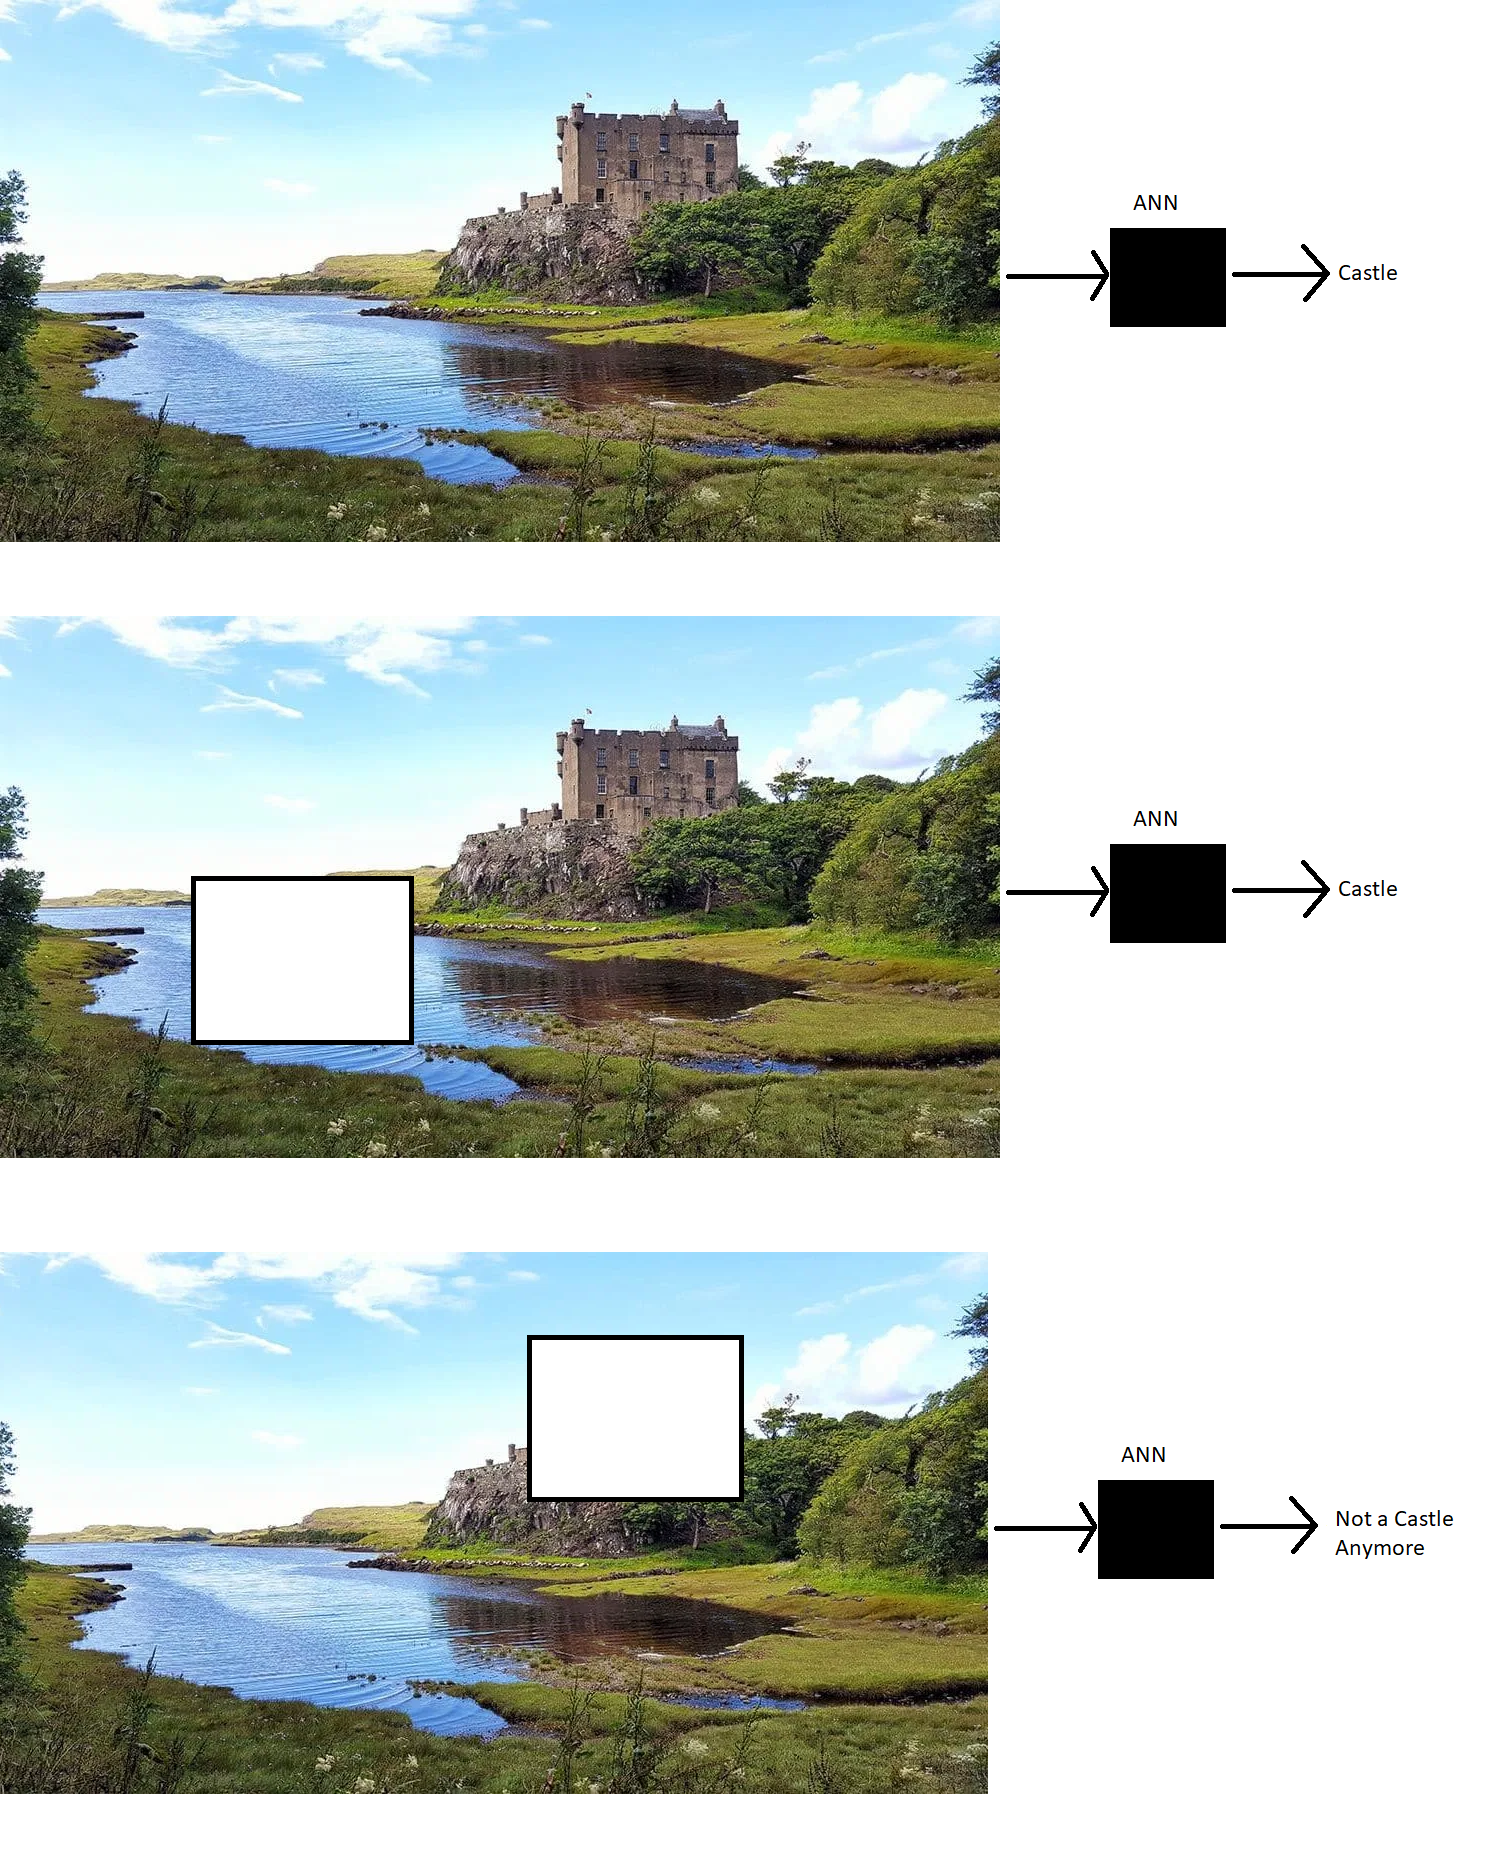
\includegraphics[width=\linewidth]{images/02_related_works/Garden-Dunvegan-Castle_Modified.png}
    \caption{Perturbation based approach visualized on an ANN trained to detect castles \cite{castle_image}}
    \label{fig:perturbation_approach}
\end{figure}

In the example above: \autoref{fig:perturbation_approach} the perturbation approach XAI tool would conclude that the pixels in the first rectangle are not important for the classification while the ones in the second one are. While seeming straight forward, this approach has two key disadvantages:

\begin{itemize}
    \item Assumes locality, \textit{meaning that it assumes that the output only depends upon the current input and the base rate of the model(the average output of the model).}
    \item Perturbations may introduce artefacts. \textit{In the above example you could imagine that a big grey rectangle is recognized if not as a castle, then at least as a concrete building. This is a particular issue when explaining text. The classifier might respond to grammatically incorrect sentences in a certain way which would be an unwanted side effect of said removal.}
\end{itemize}

\subsection{Function based approaches}

In this section we will cover the well-known Gradient x Input approach.

We will quickly reiterate some basics and then explain how this approach can be used to create an explanation. Let's say we have a classification function $f$ which takes a multidimensional input $x$. We now would like to know which direction/dimension was more important than the others. To find this dimension, we use following function: The \textit{Gradient}.

\begin{equation}
    \nabla f(x) = \frac{\delta f(x)}{\delta x}
\end{equation}

If we apply that \textit{Gradient} to $x$ like done above, we get a vector of partial derivatives of $f(x)$ for every dimension of $x$. We now know which direction has the largest impact on the classification. We can now look at that direction and determine from it which values of $x$ are the most responsible ones for the classification result. This can be done in the form of a \textit{Gradient x Input} matrix called an attribution map. For most applications, this works well but still has some issues. The gradient only tells us the importance of a dimension if we just take a tiny step which is very local information. Furthermore it suffers from \enquote{noise} (the explanation map does not form a clear structure but shows seemingly random information), an issue this thesis tries to address. This method serves as a solid conceptual basis for more involved explanation methods including the one we implemented \cite{GradientInput}.

\subsection{Surrogate-/ Sampling based approaches}

Sampling's main goal is speed. You quickly approximate a solution without guaranteeing that the solution is correct. This is a valid approach since computation power is still the biggest limiting factor concerning artificial neural networks. We will quickly look at one of these approaches: \textbf{local interpretable model-agnostic explanations (LIME)} \cite{Lime_paper}.


This method ignores the global underlying black box and only tries to provide an explanation for a single prediction. To achieve that goal, it generates a new dataset consisting of modified samples and runs them through the black box. Using this new dataset, lime then trains an interpretable model (we will come back to what an interpretable model is in \autoref{chap:basics}, for now just consider it a simple model which can be understood by just looking at its structure/code). Lime's model should be a good approximation of the original black box locally but does not have to be a good global approximation (see \autoref{fig:lime_global_local}). This kind of accuracy is called local fidelity \cite{Lime_shap_explained}. 


Throughout this thesis we will call the approximated model the \textit{explanation model} and the model we wish to explain the \textit{original model}.

\begin{figure}[H]
    \centering
    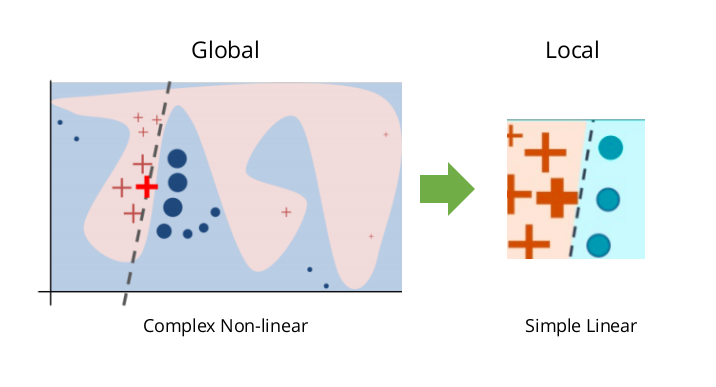
\includegraphics[width=\linewidth]{images/02_related_works/Lime_global_local.png}
    \caption{LIME localizes a problem and explains the model at that locality, rather than generating an explanation for the whole model \cite{Lime_paper}.}
    \label{fig:lime_global_local}
\end{figure}

The method we implemented, called shap, is actually a special implementation of Lime adding further rules to the algorithm making it more predictable but also less flexible. We will explain these differences in more detail in \autoref{chap:SHAP}.

\subsection{Structure based methods}

Structure based methods look at the structure of the ANN. We will briefly talk about the layer wise relevance propagation method. It tries to find subfunctions in the neural network. For example a part of the network which finds a certain pattern. We do this by starting from the output. Often, not always, we can detect a pattern, which part of the neural network is responsible to detect a certain output class. This can then be analyzed to realize what part of the input is responsible for a certain classification.\\

\begin{figure}[H]
  \centering
    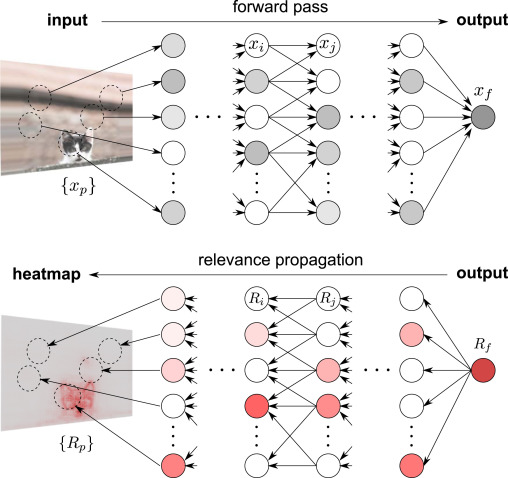
\includegraphics[width=\linewidth]{images/02_related_works/Layer wise relevance propagation2.png}
  \caption{Layer wise relevance propagation \cite{LRP}}
  \label{fig:layer_wise_relevance_prop}
\end{figure}

In \autoref{fig:layer_wise_relevance_prop} we see how the red inputs form the shape of a cat. We can then conclude, that the \enquote{activated} part of the ANN is a function detecting the shape of a cat.

This is a very powerful method with only one drawback, its implementation is very dependent on the shape of the neural network. Classifiers that do not use the traditional neural network shape cannot be analyzed using that method.

\subsection{Shap}

All of these approaches are valid, they each have their advantages and disadvantages. The method we will implement, shap, is actually a mixed approach picking tools from each basket to form a powerful explainer (\autoref{chap:SHAP}). Yet it suffers itself from a few disadvantages. We will go over in more details about those and how our work tries to address one of these issues (\autoref{ch:Results}).